\documentclass[12pt]{article}

%%%%%%%%%%%%PACKAGES%%%%%%%%%%%%%%
\usepackage[top=2cm,bottom=2cm, right = 1cm, left = 1.5cm]{geometry}
\usepackage{fancyhdr}

\usepackage[T2A]{fontenc}
\usepackage[english, russian]{babel}
\usepackage{tempora}% bold titles and nice style
\usepackage{graphicx}%%%allow inserting images
\usepackage{xcolor}
\usepackage{enumitem}
\usepackage{float}
%%%%%%%%%%%%%%%%%%%%%%%%%%%%%%%%%

%%%%%%%%%%%%%%%%%%%%%%%%%%preambules%%%%%%%%%%%%%%%%%%%%
%%%%%%%%%%%%%%%%%%%%%%%%%%%%%%%%%%%%%%%%%%%%%%%%%%%%%%%%

\pagestyle{fancy}
\fancyhead{}
\fancyfoot{}%clear all the footnotes
\fancyhead[L]{\slshape\MakeUppercase{РУДН}}
\fancyhead[R]{\slshape{python}}
\fancyfoot[C]{\thepage}%set the notes as the page number
\setlength{\parskip}{0.5em} %lenght between paragrahs
\renewcommand{\baselinestretch}{1.2}%spacing between lines
\parindent 0ex %remove the espace of the first line in every paragraph

%%%%%%%%%%%%%%%%%%%%%%%%%%custom colors%%%%%%%%%%%%%%%%%%%%%%%%%%
%%%%%%%%%%%%%%%%%%%%%%%%%%%%%%%%%%%%%%%%%%%%%%%%%%%%

\usepackage{listings}
\definecolor{codegreen}{rgb}{0.1,0.7,0.1}
\definecolor{codegray}{rgb}{0.5,0.5,0.5}
\definecolor{codepurple}{rgb}{0.7,0,0.98}
\definecolor{codemagenta}{rgb}{1,0,1}
\definecolor{backcolour}{rgb}{1,1,1}
\definecolor{aqua}{rgb}{0.0, 1.0, 1.0}
\definecolor{myyellow}{rgb}{0.9, 0.9, 0.0}

%%%%%%%%%%%%%%%%%%%%%%%%%listing styles%%%%%%%%%%%%%%%%%%%%%%%%%%
%%%%%%%%%%%%%%%%%%%%%%%%%%%%%%%%%%%%%%%%%%%%%%%%%%%%

\usepackage{listings}

\lstdefinestyle{conlst}{
	morekeywords={[1] .py},
	keywordstyle={ [1]\color{orange} },
	basicstyle=\Large\ttfamily,
	commentstyle=\color{gray} \emph,
	stringstyle=\ttfamily,
	backgroundcolor=\color{backcolour},
	stringstyle=\color{codegreen},
	showspaces=false,
	showtabs=false,
	breaklines=true,
	showstringspaces=false,
	breakatwhitespace=true,
	upquote=true,
	frame=tblr,
	escapechar =@,
	columns=fullflexible
	%aboveskip=20pt,
	%belowskip=20pt
	}

\lstdefinestyle{pylst}{
	language=Python,
	morekeywords={[1] None, True, False},
	morekeywords={[2] __init__, __name__},
	morekeywords={[3] self},
	basicstyle=\Large\ttfamily,
	keywordstyle={[1]\color{blue}},
	keywordstyle={[2]\color{codemagenta}},
	keywordstyle={[3]\color{codepurple}},
	keywordstyle={[4]\color{codegreen}},
	commentstyle=\color{codegreen} \emph,
	%stringstyle=\ttfamily,
	numbers=left,
	numberstyle=\small, 
	stepnumber=1, 
	numbersep=5pt,
	backgroundcolor=\color{backcolour},
	stringstyle=\color{orange},
	showspaces=false,
	showtabs=false,
	breaklines=true,
	showstringspaces=false,
	breakatwhitespace=true,
	upquote=true,
	frame=tblr,
	escapechar =@,
	columns=fullflexible,
	%aboveskip=20pt,
	%belowskip=20pt
	}

\lstset{literate=%
   *{0}{{{\color{codegreen}0}}}1
    {1}{{{\color{codegreen}1}}}1
    {2}{{{\color{codegreen}2}}}1
    {3}{{{\color{codegreen}3}}}1
    {4}{{{\color{codegreen}4}}}1
    {5}{{{\color{codegreen}5}}}1
    {6}{{{\color{codegreen}6}}}1
    {7}{{{\color{codegreen}7}}}1
    {8}{{{\color{codegreen}8}}}1
    {9}{{{\color{codegreen}9}}}1
}

%%%%%%%%%%%%%%%%%%%%%%%%%%%%%%%%%%%%%%%%%%%%%%%%%%%%%%%%%%
%%%%%%%%%%%%%%%%%%%%%%%%%%%%%%%%%%%%%%%%%%%%%%%%%%%%%%%%%%
\begin{document}
\tableofcontents
\newpage
\setcounter{page}{1}%set this page as the first page
\section{Требования}
\begin{enumerate}
	\item подключение к интернету
  \item интернет браузер
\end{enumerate}

\section{Создание учетной записи в pythonAnyWhere}
	\begin{enumerate}
    \item перейдите по следующей ссылке:
      \begin{lstlisting}[caption=\phantom{},style=conlst,label={lst:enter_desktop}]
      https://www.pythonanywhere.com/pricing/
			\end{lstlisting}

    \item нажмите кнопку «create a beginner account»
	\begin{figure}[H]
		\centering
		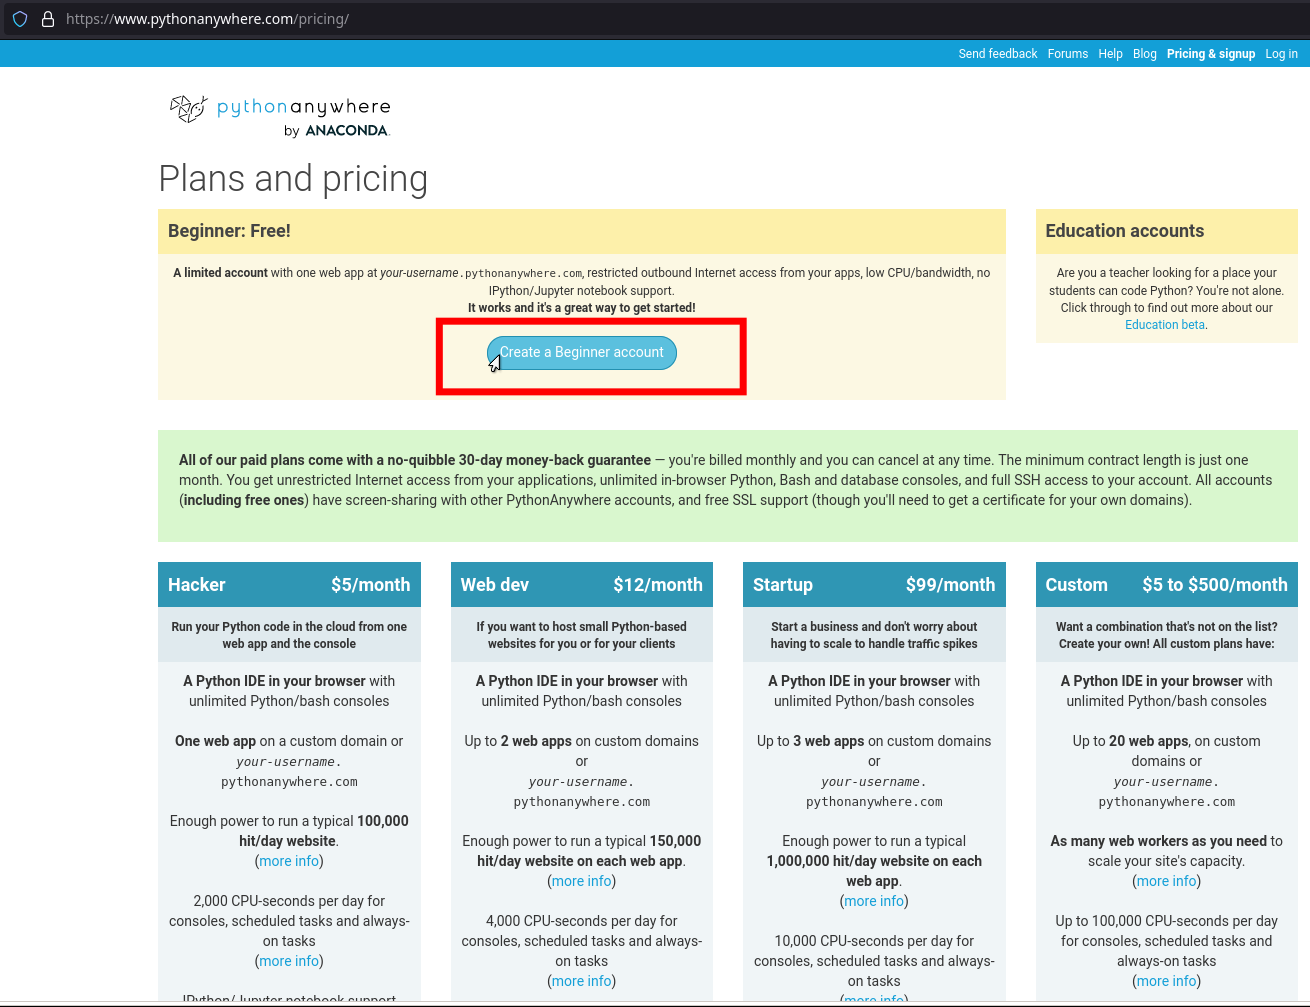
\includegraphics[width=0.8\textwidth ,keepaspectratio]{imgs/create_beginner_account.png}
		\caption{}
	\end{figure}

    \item заполните всю необходимую информацию и нажмите «register». Пожалуйста, следуйте рекомендациям:
      \begin{itemize}
        \item вы ДОЛЖНЫ иметь доступ к электронной почте, которую вы используете при регистрации.
        \item запомните свое имя пользователя и пароль, они понадобятся вам позже.
          \end{itemize}
	\begin{figure}[H]
		\centering
		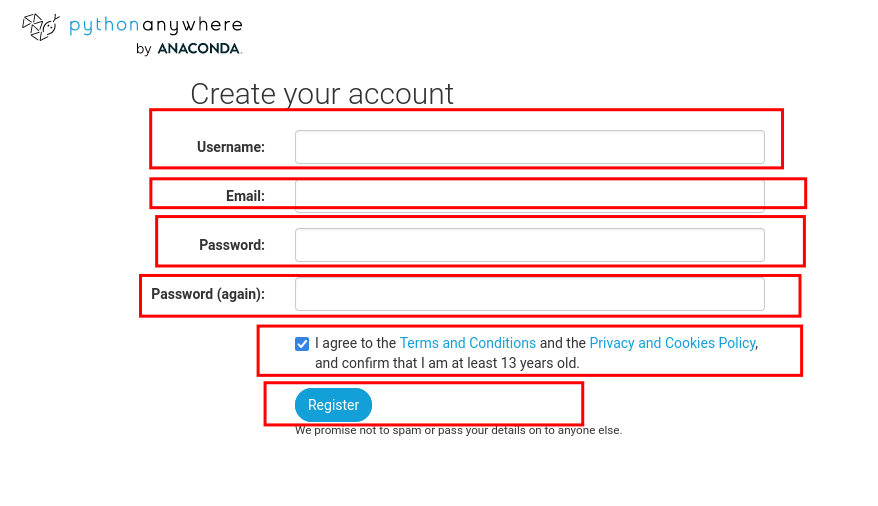
\includegraphics[width=0.8\textwidth ,keepaspectratio]{imgs/fill_reg_info.png}
		\caption{}
	\end{figure}
	\end{enumerate}
\section{Создание виртуальной среды}

	\begin{enumerate}
    \item открыть терминал
	\begin{figure}[H]
		\centering
		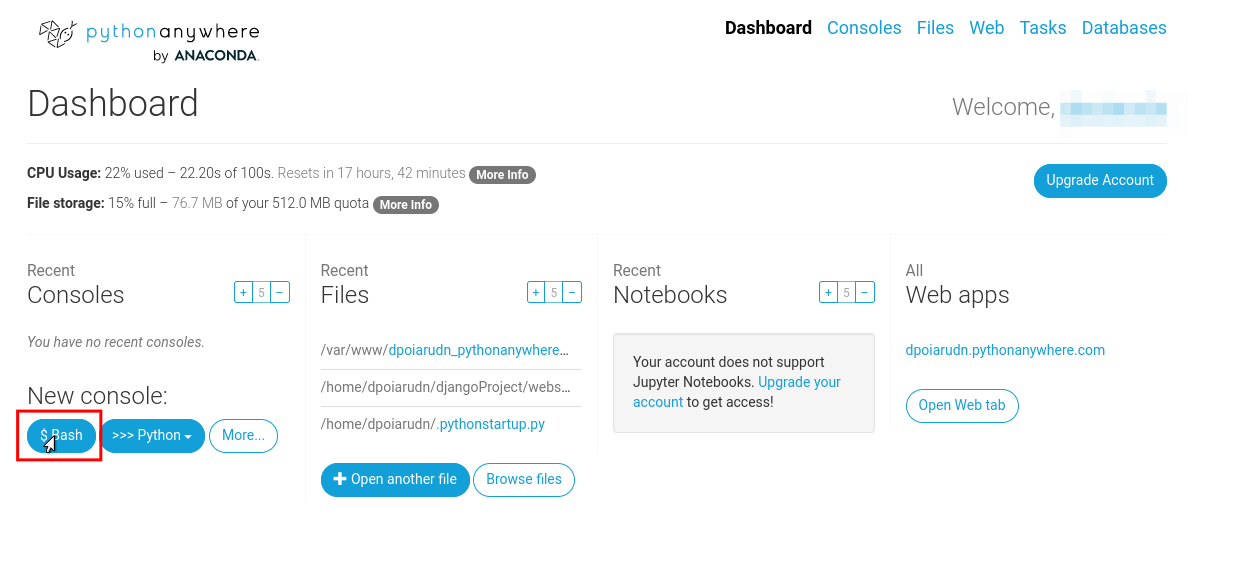
\includegraphics[width=1.0\textwidth ,keepaspectratio]{imgs/open_terminal.png}
		\caption{}
	\end{figure}

    \item убедитесь, что у вас установлен python
			\begin{lstlisting}[caption=\phantom{},style=conlst,label={lst:enter_desktop}]
      python --version
			\end{lstlisting}
	\begin{figure}[H]
		\centering
		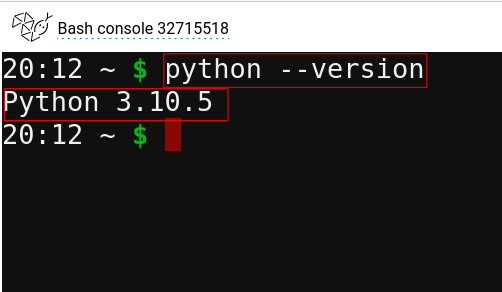
\includegraphics[width=0.3\textwidth ,keepaspectratio]{imgs/verify_py_version.png}
		\caption{}
	\end{figure}

    \item создать виртуальную среду
			\begin{lstlisting}[caption=\phantom{},style=conlst,label={lst:enter_desktop}]
python -m venv djangoEnv
			\end{lstlisting}
	\begin{figure}[H]
		\centering
		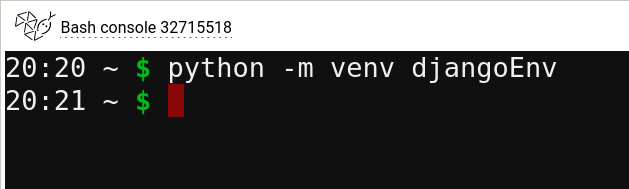
\includegraphics[width=0.4\textwidth ,keepaspectratio]{imgs/create_venv.png}
		\caption{}
	\end{figure}

    \item убедитесь, что новая виртуальная среда создана
			\begin{lstlisting}[caption=\phantom{},style=conlst,label={lst:enter_desktop}]
      ls -1
			\end{lstlisting}
	\begin{figure}[H]
		\centering
		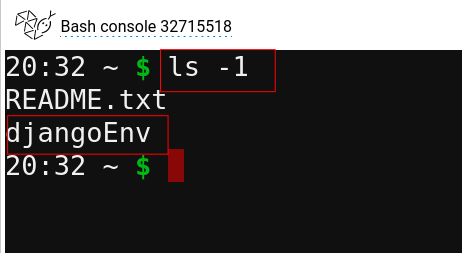
\includegraphics[width=0.3\textwidth ,keepaspectratio]{imgs/check_venv_creation.png}
		\caption{}
	\end{figure}
	\end{enumerate}

\section{Установка django}
	\begin{enumerate}
    \item войти в папку виртуальной среды
			\begin{lstlisting}[caption=\phantom{},style=conlst,label={lst:enter_desktop}]
      cd djangoEnv/
			\end{lstlisting}
	\begin{figure}[H]
		\centering
		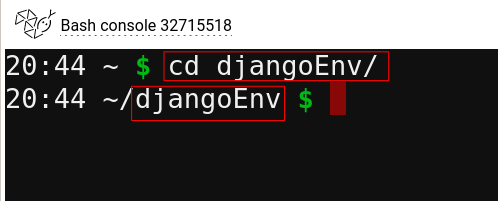
\includegraphics[width=0.4\textwidth ,keepaspectratio]{imgs/enter_venv_folder.png}
		\caption{}
	\end{figure}

    \item активировать виртуальную среду
			\begin{lstlisting}[caption=\phantom{},style=conlst,label={lst:enter_desktop}]
      source bin/activate
			\end{lstlisting}
	\begin{figure}[H]
		\centering
		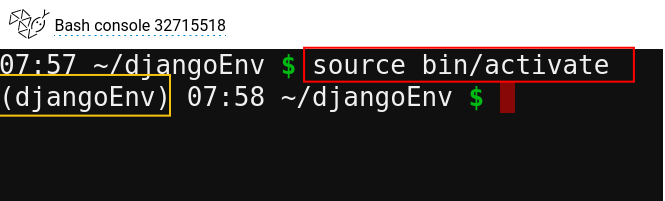
\includegraphics[width=0.5\textwidth ,keepaspectratio]{imgs/activate_venv.png}
		\caption{}
	\end{figure}

    \item установить django
			\begin{lstlisting}[caption=\phantom{},style=conlst,label={lst:enter_desktop}]
      pip install django
			\end{lstlisting}
	\begin{figure}[H]
		\centering
		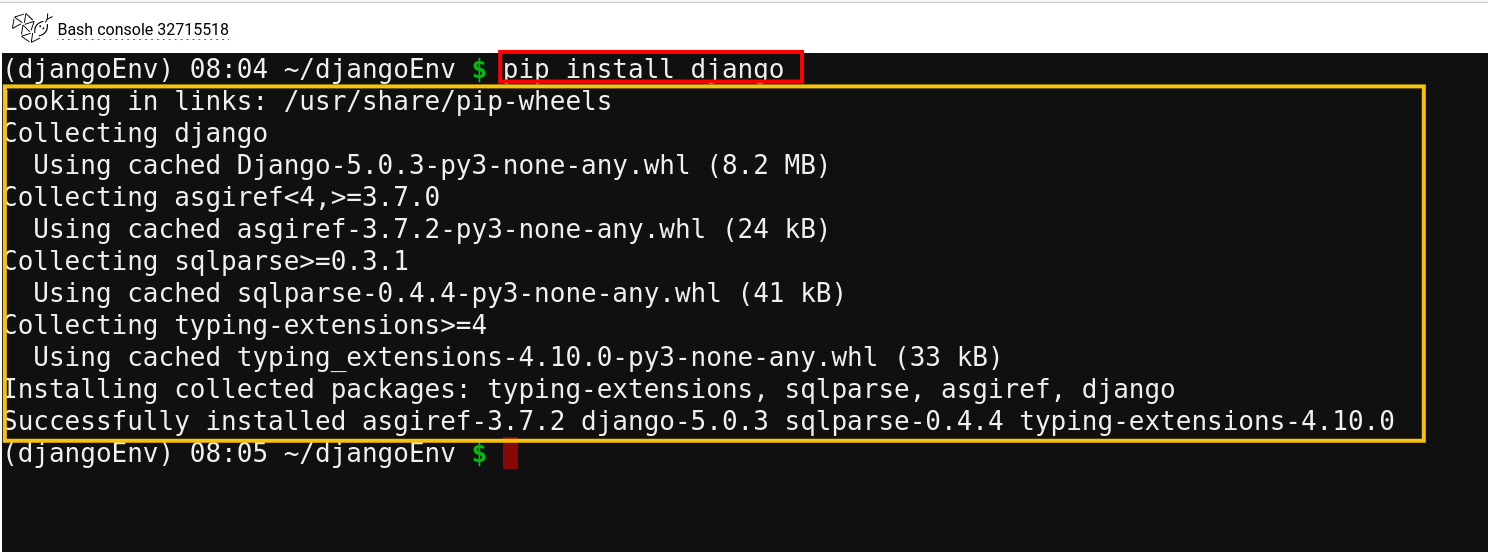
\includegraphics[width=0.7\textwidth ,keepaspectratio]{imgs/install_django.png}
		\caption{}
	\end{figure}

    \item проверьте, установлен ли django
			\begin{lstlisting}[caption=\phantom{},style=conlst,label={lst:enter_desktop}]
      pip list
			\end{lstlisting}
	\begin{figure}[H]
		\centering
		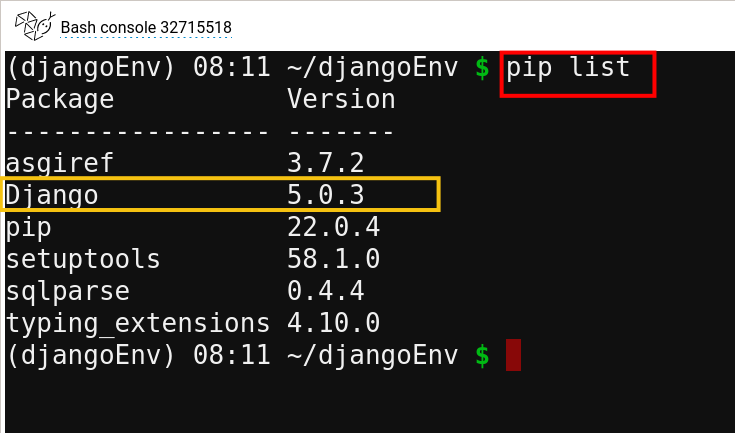
\includegraphics[width=0.5\textwidth ,keepaspectratio]{imgs/check_django_installation.png}
		\caption{}
	\end{figure}

    \item выйти из терминала
			\begin{lstlisting}[caption=\phantom{},style=conlst,label={lst:enter_desktop}]
      exit
			\end{lstlisting}
	\begin{figure}[H]
		\centering
		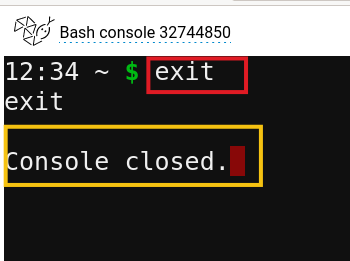
\includegraphics[width=0.3\textwidth ,keepaspectratio]{imgs/exit_terminal.png}
		\caption{}
	\end{figure}
	\end{enumerate}
\end{document}
